% !TEX root = ../main.tex
\section{Motivation}
\label{sec:mot}

We study the MoE layers of Qwen3-30B-A3B compiled for the four SoCs of one Cloud AI 100 Ultra card (setup in
\S\ref{sec:setup}). The exported graph \citep{qefficient} runs a layer's 128 experts as two stages of 64 \emph{lanes}; a
lane is one expert's gate, up and down GEMMs over a fixed number of gathered token rows, its capacity $C$. The production
program uses $C=T$, the only capacity that never drops a token. Three questions motivate \sys: why capacities should
follow the load at run time, why that is not enough without efficient aggregation, and why the graph's expression of the
aggregation decides its cost.

\subsection{Expert Loads Vary, and Padding Is Executed Work}
\label{sec:mot-pad}

We captured the routing of all 48 layers for 50 prompts of 128 tokens from each of eight workloads, GSM8K, MMLU,
SWE-bench Lite issues, HumanEval and its JavaScript version, Alpaca instructions, CNN/DailyMail articles and Chinese XNLI
sentence pairs \citep{cobbe2021gsm8k,hendrycks2021mmlu,jimenez2024swebench,chen2021humaneval,muennighoff2024octopack,taori2023alpaca,hermann2015cnndm,conneau2018xnli},
and for chunks of 256 and 512 tokens from four of them (Appendix~\ref{app:calib}). The load is skewed, with one expert of
some layer receiving 127 of 128, 256 of 256 and 508 of 512 tokens, and the skew is workload-specific: across workloads the
16 most loaded experts of a layer agree with a Jaccard index of 0.00--0.33, against 0.52--0.88 between the two halves of
one workload.

\begin{figure}[t]
\centering
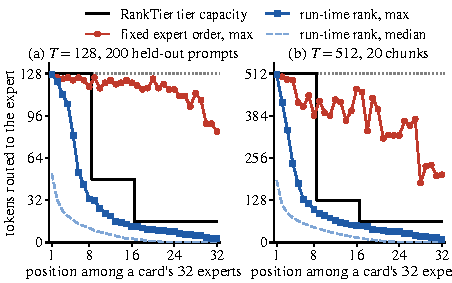
\includegraphics[width=\columnwidth]{figures/fig_rank_identity.pdf}
\vskip -0.08in
\caption{Rows a SoC must reserve for its expert at each position, as the largest load observed there. Red: experts in a
fixed order, ranked by their mean load on calibration prompts (a: the first half of each workload's prompts, evaluated on
the other half; b: leave-one-out over the chunks). Blue: experts ordered at run time by their load in the chunk itself.
Black: \sys's tier capacities. Dotted: capacity $T$.}
\label{fig:rank}
\vskip -0.1in
\end{figure}

A program that fixes which lane serves which expert must reserve at each lane the largest load its expert can receive.
Ordering each SoC's 32 experts by their mean load on calibration prompts, the held-out maximum is 84--127 of 128 rows at
\emph{every} position (Figure~\ref{fig:rank}): a drop-free fixed layout needs 91\% of the rows of padding everything to $T$.
Ordered by their load in the chunk itself, the same experts need far less below the first ranks: the 16th most loaded
expert of a SoC never received more than 12 of 128 tokens.

Allocated rows matter only if they are executed. The compiler has no data-dependent control flow, but it predicates each
row tile of a lane on whether the tile holds a routed token (\S\ref{sec:skip}): a lane with $n$ tokens and row tile $R$
computes $R\lceil n/R\rceil$ rows, and skips its weights only when it is a single tile. At $T=512$ the static
capacity-$T$ program computes 13.8--15.4k of its 16.4k rows per SoC at the default tile size and still 3.5--3.8k at the
smallest one the compiler accepts. Executed padding costs time once the chunk is long: the tensor-unit time of a SoC's 16
most loaded experts is 44, 310 and 921\,\textmu s per core at capacities 92, 158 and 296, 21$\times$ for 3.2$\times$ the
rows, while their weight stream stays constant.

\subsection{Capacity Savings Need Efficient Aggregation}
\label{sec:mot-red}

After the expert GEMMs, each expert's rows return to their tokens, are weighted and summed over the token's experts and
then across devices. The exported graph does this densely: each stage scatters its rows into a zero-filled accumulator of
shape $[\mathrm{lanes},T,d]$, sums it over each SoC's lanes and sums the four SoC partials, a cost that grows with
lanes$\,\times\,T$ whatever the routing. Ranked capacities change this step's inputs: tiers of different widths produce
differently shaped outputs in more stages, and a lane-dense accumulator is needed per width.

\begin{figure}[t]
\centering
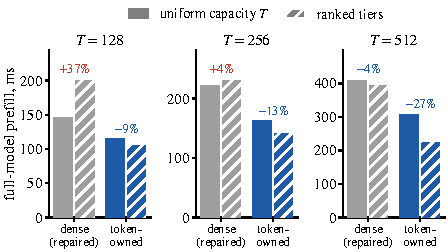
\includegraphics[width=\columnwidth]{figures/fig_interaction.pdf}
\vskip -0.08in
\caption{Capacity $\times$ aggregation. Full-model prefill latency with uniform capacity $T$ and with \sys's ranked tiers,
under the repaired dense combine and under token-owned aggregation. All four programs rank experts at run time, gather
their weights from the same bank and use the same final sum and tile size; percentages are latency changes from tiering.}
\label{fig:interaction}
\vskip -0.1in
\end{figure}

Figure~\ref{fig:interaction} holds everything else fixed and varies only the capacities and the aggregation. The dense
baseline is repaired: its accumulators are not read back after zero-filling, and its lane sums run in token tiles
(\S\ref{sec:impl}). Under it, ranked tiers change full-model latency by $+37\%$, $+4\%$ and $-4\%$ at $T=128$, 256 and 512;
under token-owned aggregation, by $-9\%$, $-13\%$ and $-27\%$. The rows the tiers save are the same in both. Minimizing
padded expert work is therefore an incomplete objective: capacity selection must be designed together with aggregation.
The repaired dense combine does gain from tiers at $T=512$, so the claim is about the size and consistency of the benefit,
not about whether any benefit exists.

\subsection{Equivalent Arithmetic, Different Placement}
\label{sec:mot-own}

The aggregation \sys needs is a standard sparse combine: each device gathers the rows of the experts it computed for each
token, sums them into a per-token partial, and the partials are summed across devices
(\S\ref{sec:bg}). A graph compiler, though, decides from the graph's form where each part runs. Figure~\ref{fig:ownership}
compares three graphs that compute exactly this sum, with the same index values, summation order and final sum, and
produce bit-identical logits; they differ only in how they express which SoC owns which expert rows. Addressing each SoC's
rows by global row indices into the stage's unsplit outputs, or cutting each SoC's lanes out with explicit slices, makes the
compiler move expert outputs between SoCs, 1539\,MiB per MoE layer against 14\,MiB, and runs the full model 4.4--5.3$\times$
and 3.4--4.1$\times$ slower. A reshape that exposes the SoC partition the compiler already applies to the lane axis as the
leading batch axis of the gather keeps every row on its device. With arithmetic and outputs held constant, the alternative
expressions cause far more redistribution and much higher latency; they may also change scheduling, buffering or tiling,
which the experiment does not separate.

\begin{figure}[t]
\centering
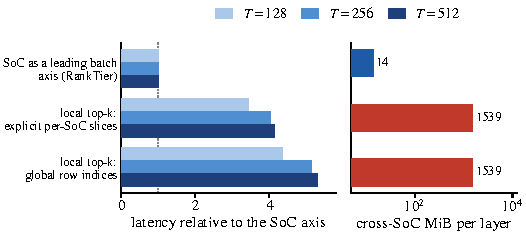
\includegraphics[width=\columnwidth]{figures/fig_ownership.pdf}
\vskip -0.08in
\caption{Equivalent arithmetic, different placement. Three expressions of the same per-SoC token aggregation, with
bit-identical logits. Left: full-model latency relative to the layout-preserving SoC axis. Right: cross-SoC traffic inside
one MoE layer at $T=512$, from instrumented two-layer profiles.}
\label{fig:ownership}
\vskip -0.1in
\end{figure}

Ownership is the first requirement; the second is local reduction. A token's expert rows can sit on several cores of a
SoC, and a formulation that keeps device locality but sums over the lanes of every token tile pulls its operands from all
16 cores, 242\,MiB of cross-core traffic per layer, and is 11--15\% slower than summing each token's rows on the core that
owns the token (\S\ref{sec:eval-own}). Expressing a top-$k$ gather is therefore an incomplete implementation: the graph
must preserve device ownership when it selects expert outputs, and assign each token's reduction to one core.
